\chapter{Dataless neural network structure for maximum independent set problem}

Usually in classical supervised learning neural networks we have a training dataset that consists of input layer $x \in R^n$ and output layer $y \ in R^k$. The goal of the learning to update neural network weights $\theta$ in such way that difference between desired outputs and networks' outputs have at least difference as possible.  

Neural network for this particular problem does not use supervised learning and consists of input layer, 2 hidden layers and output layer. Assuming that network should not have any train data it's structure has to be dependent only on the graph structure. Thus, all layers should be derived from the graph parameters (vertices and edges). Let's denote number of vertices in the \graphG as $n$ and the number of edges as $m$. Training parameters $\theta$ consists of $n$ binary parameters $\{0,1\}$: $\theta \in \{0,1\}$. After the training process $\theta_i$ should be equal to $1$ if vertex $v_i:v_i \in V$ should be included in independent set and $0$ otherwise. Training weights form first hidden layer of the network. Input layer is 1-dimensional vector $e_n$ where all values are equal to 1. Input layer is connected to training weights by element-wise product. Edges structure of the graph is represented by the second hidden layer. The second hidden layer is described by binary matrix $W \in \{0,1\}^{n(n+m)}$ and the bias vector $b \in \{-1,-1/2\}^{n+m}$ and rectified linear activation function ReLU. 

The second hidden layer is connected to the output  layer by vector $\omega \in \{-1,n\}^{n+m}$ using element-wise product $\sigma (x) = max(0,x)$. Final formula for the output of the neural network is 
\begin{equation}
    f(e_n;\theta) = f(\theta) = \omega^T \sigma(W\theta(e_n \odot \theta)+b)
\end{equation}
Parameters of $f$ are constructed from the graph \graphG with next approach:
First $n x n$ submatrix of $W$ represents the vertices of $V$ in the graph and it's values are equal to the identity matrix $I_n$ such that $W_{i,j} = 1, \forall i = \overline{0, n-1}$. Next $m$ columns of $W$ are used to represent the edges $E$ in the graph. 

\begin{equation} 
W =
\begin{bmatrix} 
1 & 0 & 0 & \cdots & 0 & W_{1,n+1} & W_{1,n+2} & \cdots & W_{1, n+m} \\ 
0 & 1 & 0  & \cdots & 0 & W_{2,n+1} & W_{2,n+2} & \cdots & W_{2, n+m} \\ 
% 0 & 0 & 1 & \cdots & \vdofpicts & \vdots & \ddots & & \vdots \\
\vdots & \vdots & \vdots & \ddots & \vdots & \vdots & \vdots & \ddots & \vdots \\
0 & 0 & 0 & \cdots & 1 & W_{n, n+1} & W_{n, n+2} & \cdots & W_{n, n+m}
\end{bmatrix}
\end{equation}

where $W_{i,n+l} = W_{j,n+l} = 1, \forall e_l = (v_i, v_j) \in E, l\in [m] $ 

\newtheorem{theorem}{Theorem}
\begin{theorem}
\label{minimum_f_value_theorem}
Given a graph \graphG and it's neural network f, maximum independent set $I \subseteq V$ of $G$ has size $|I| = k \iff$ minimum value of $f$ is $-k/2$. 
\end{theorem}
\begin{proof}
$(\Longrightarrow)$
Assume that $|U| = k$ and let $\theta_{v_i} = 1, \forall v_i \in U$ and $\theta_{v_i} = 0$ otherwise. For an arbitrary pair of nodes $v_i, v_j \in U$, consider the output of $f$ where edge values denote the outputs of the preceding nodes in the network and nodes ${\mu_i}^1, {\mu_i}^2$ denote the $i^{th}$ neurons in the first and second hidden layers, respectively. We abuse notation to refer to both the output neuron and the output value as $f(\theta)$.

Note that $v_i$ and $v_j$ each contribute an output of -1/2 to $f(\theta)$. This follows from the fact that, by definition of MIS, these vertices do not share an edge and so the output of ${mu^2}_{n+l}$ is 0.
Thus, for an MIS of size $|U| = k$,
we have $f(\theta)=-k/2$.
This is the minimum value attainable by $f$. 


Indeed, consider, for the sake of contradiction, that there exists $\theta'$ such that $f(\theta') < f(\theta)$. 
As with $\theta$, this $\theta'$ must be defined such that $\theta_{v_i} = 1 \forall v_i \in U$. Consider the addition of some other $v_{k'} \notin U$. Then ${\mu_{k'}}^2$ will contribute $-\sigma(\theta_{k'}-1/2$ to $f(\theta')$ 
and ${\mu^2}_{n+l}$ will contribute at least $n\theta_{k'}$ for every edge $e_k = (v_{k'}, v) \in E$, where $v \in U$. By definition of MIS, some such edge must exist. Therefore, we would have $f(\theta) > f(\theta)$, yielding a contradiction.

$(\Longleftarrow)$ Assume that the minimum value of $f$ is $f(\theta) = -k/2.$ Consider an arbitrary edge $e_l = (v_i, v_j) \in E$. It follows from the construction of $f$ that $\theta_{v_i} + \theta_{v_j} \leq 1$ must hold for $f$ to achieve its minimum value. To obtain contradiction, let $\theta_i + \theta_j > 1$, then ${\mu^2}_{n+l}$ contributes $n(\theta_i+\theta_j-1)>0$ to the result of $f(\theta)$. This causes contradiction as we can choose $\theta_i$ and $\theta_j$ to be 0, contributing a value of 0 to $f(\theta)$. 
Given a vertex $v$ and its neighbors $N(v)$, $\theta_i$ must be equal to 1 for
some $v_i \in N(v)$ as this would contribute a value of -1/2 to
$f(\theta)$ through node ${\mu^2}_i$ and a value of 0 through nodes ${\mu^2}_{n+l} \forall u \in N(v)$ that
are connected to $v$ with the edge $e_l$. Because of this there must be $k$ entries in $\theta$ with value 1, with corresponding contribution value -1/2 to the output $f(\theta)$ such that none of them share a neuron in the second layer. This leads to $k$ nodes in $V$ that don't have common edge. Thus, $|U| = k$. 
\end{proof}

Minimum value of $f$ is obtained when the maximum amount of vertices in $\theta$ have value 1 and there are no edges between them. This forms an independent set 
\begin{equation}
    I(\theta) = \{ v_i \in V | \theta_{v_i} \}
\end{equation}
 of the maximum cardinality. 
 
Overall, the scheme of the proposed dataless neural network is shown on picture \ref{fig:dnn_scheme}. Example of neural network for particular graph is shown on the picture \ref{fig:dnn_example_1}.

 \begin{figure}[H]
    \centering
    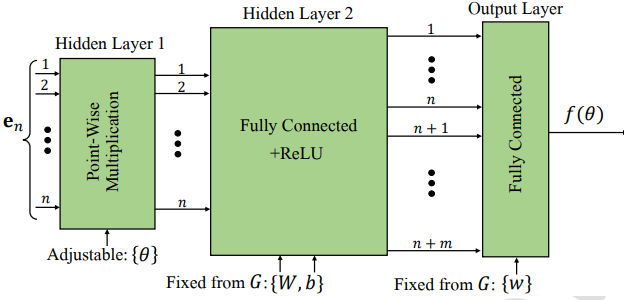
\includegraphics{figures/nn_block_structure.png}
    \caption{Scheme of proposed neural network $f(\theta)$}
    \label{fig:dnn_scheme}
\end{figure}

\begin{figure}[H]
    \centering
    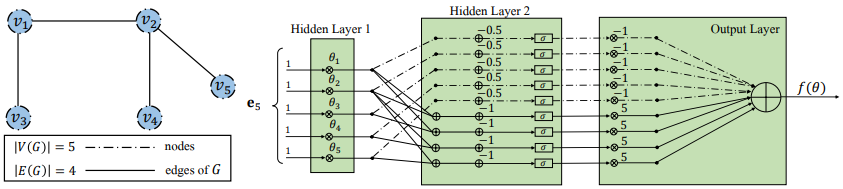
\includegraphics{figures/dnn_example.png}
    \caption{ An example of graph $G = (V = {v_1, v_2, v_3, v_4, v_5}, E =
{(v_1, v_2), (v_1, v_3), (v_2, v_4), (v_2, v_5)})$ and its dNN construction f for the MIS problem}
    \label{fig:dnn_example_1}
\end{figure}

\subsection{Loss function minimization techniques}
For minimization of the function and training the network we can use a few different approaches, like gradient descent, evolutionary minimization etc. 
 In our study we try to use both gradient descent approach and evolutionary minimization.
\subsubsection{Gradient descent}
 The main idea of gradient descent is to compute the gradient of the function and then apply a small step in the direction of the function minimization.
 For this it is relevant to imagine weights and biases stored as a 1-dimensional vector that we can call $\textbf{p} \in \mathbb{R}$.
Let the $\alpha (p):\mathbb{R}^s\ \longrightarrow \mathbb{R}$ be the loss function.
The process is iterative and involves computing a series of vectors in Rs with the goal of minimizing the loss function. Let us suppose that our current vector is \textbf{$p$}: how should we choose a perturbation,
$\delta p$, so that the next vector, $p+ \delta p$, represents an improvement? A Taylor series expansion
gives:
$$
\mathcal{L}(\mathbf{p}+\Delta \mathbf{p}) \approx \mathcal{L}(\mathbf{p})+\sum_{r=1}^s \frac{\partial \mathcal{L}(\mathbf{p})}{\partial p_r} \Delta p_r
$$
Here $ \frac{\partial \mathcal{L}(\mathbf{p})}{\partial p_r} $ stands for the partial derivative of the loss function with respect to $\textit{r}$-th parameter.  For convenience, we will let $\Delta \mathcal{L}(\mathbf{p}) \in \mathbb{R}^s$ denote the vector of partial derivatives,
known as the \textit{gradient}, so:
$$
\mathcal{L}(\mathbf{p}+\Delta \mathbf{p}) \approx \mathcal{L}(\mathbf{p})+\Delta \mathcal{L}(\mathbf{p})^T \Delta \mathbf{p}
$$
Our aim is to reduce the value of the loss function, so we should choose $\Delta \mathbf{p}$ to make $\Delta \mathcal{L}(\mathbf{p})^T \Delta \mathbf{p}$ as negative as possible. Hence, we should choose $\Delta \mathbf{p}$ to lie in the direction $-\Delta \mathcal{L}(\mathbf{p})$, limiting ourselves to a small step in that direction. This leads to the update:
$$
\mathbf{p} \longrightarrow \mathbf{p}-\eta \Delta \mathcal{L}(\mathbf{p})
$$
Here, $\eta$ is an optimization hyperparameter known as the learning rate, which controls the size of the step that the parameters take in the direction of the gradient.

However, when we have a large number of parameters and a large number of training points, computing the gradient vector at every iteration of the gradient descent method can be prohibitively expensive. A much cheaper alternative is to replace the mean of the individual gradients over all training points by the gradient at a single, randomly chosen, training point. This leads to the simplest form of what is called the stochastic gradient method (SGD) \ref{fig:gradient_descent}.

\begin{figure}[h]
    \centering
    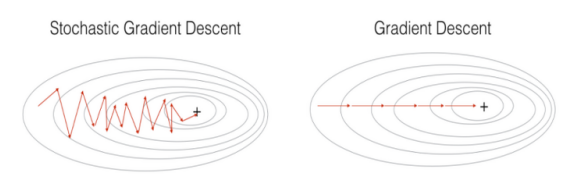
\includegraphics{figures/gradient_descent.png}
    \caption{Gradient descent}
    \label{fig:gradient_descent}
\end{figure}
 
 For gradient descent complexity of the algorithm depends on complexity of the gradient calculation. Noticing, that in network all parameters except $\theta$ are fixed, we can calculate only one gradient $\nabla |f(\theta) - f_d|^2$. Other parameters describe only the graph structure and are constant during the training procedure so they don't have to be updating by the gradient applying phase. 
 Thus, we iteratively minimize the loss function $\mathcal{L}(f(\theta),f_d)=|f(\theta)-f_d|^2$ by applying the gradient descent. 
 According to the Theorem \ref{minimum_f_value_theorem}, the minimum achievable value of $f(\theta)$ is a function of the cardinality of MIS. According to this, we set $f_d=n/2$ because we don't now what is the size of the MIS.

\subsubsection{Evolutionary minimization}

Because they ideally make no assumptions about the underlying fitness landscape, evolutionary algorithms frequently do well in approximating solutions to many kinds of problems. Planning models based on cellular processes and investigating microevolutionary processes are the main applications of evolutionary algorithms to the modeling of biological evolution. Computational complexity is a limiting issue in the majority of real-world implementations of EAs. Actually, the assessment of the fitness function is what causes this computational complexity. One method to get around this problem is to approximate fitness. There may not be a straight correlation between algorithm complexity and issue complexity, as seeming simplicity in EA can solve complicated problems frequently.

For our study we use a variant of \textbf{differential evolution}.

A basic variant of the DE algorithm works by having a population of candidate solutions (called agents). These agents are moved around in the search-space by using simple mathematical formulae to combine the positions of existing agents from the population. If the new position of an agent is an improvement then it is accepted and forms part of the population, otherwise the new position is simply discarded. The process is repeated and by doing so it is hoped, but not guaranteed, that a satisfactory solution will eventually be discovered.

Formally, let $f: \mathbb{R}^n \rightarrow \mathbb{R}$ be the fitness function which must be minimized (note that maximization can be performed by considering the function $h:=-f$ instead). The function takes a candidate solution as argument in the form of a vector of real numbers and produces a real number as output which indicates the fitness of the given candidate solution. The gradient of $f$ is not known. The goal is to find a solution $\mathbf{m}$ for which $f(\mathbf{m}) \leq f(\mathbf{p})$ for all $\mathbf{p}$ in the search-space, which means that $\mathbf{m}$ is the global minimum.

Let $\mathbf{x} \in \mathbb{R}^n$ designate a candidate solution (agent) in the population. The basic DE algorithm can then be described as follows:
\begin{enumerate}
\item Choose the parameters $\mathrm{NP} \geq 4, \mathrm{CR} \in[0,1]$, and $F \in[0,2]$
    \begin{enumerate}
        \item $\mathrm{NP}$ is the population size, i.e. the number of candidate agents or "parents"; a typical setting is $10 n$
        \item The parameter $\mathrm{CR} \in[0,1]$ is called the crossover probability and the parameter $F \in[0,2]$ is called the differential weight. Typical settings are $F=0.8$ and $C R=0.9$.
    \end{enumerate}
    \item Initialize all agents $\mathbf{x}$ with random positions in the search-space.
    \item Until a termination criterion is met (e.g. number of iterations performed, or adequate fitness reached), repeat the following:
    \begin{enumerate}
        \item Pick three agents $\mathbf{a}, \mathbf{b}$, and $\mathbf{c}$ from the population at random, they must be distinct from each other as well as from agent $\mathbf{x}$. (a is called the "base" vector.)
        \item Pick a random index $R \in\{1, \ldots, n\}$ where $n$ is the dimensionality of the problem being optimized.
        \item Compute the agent's potentially new position $\mathbf{y}=\left[y_1, \ldots, y_n\right]$ as follows:
        \begin{enumerate}
        \item For each $i \in\{1, \ldots, n\}$, pick a uniformly distributed random number $r_i \sim U(0,1)$
        \item If $r_i<C R$ or $i=R$ then set $y_i=a_i+F \times\left(b_i-c_i\right)$ otherwise set $y_i=x_i$. (Index position $R$ is replaced for certain.)
        \end{enumerate}
        \item If $f(\mathbf{y}) \leq f(\mathbf{x})$ then replace the agent $\mathbf{x}$ in the population with the improved or equal candidate solution $\mathbf{y}$
    \end{enumerate}
    \item Pick the agent from the population that has the best fitness and return it as the best found candidate solution.
\end{enumerate} 

 
\section{Exploiting the max clique problem in the neural network}
 
 We suggest including the edges of $G'$ since the graph generated by the MIS is a null graph on G and completely connected on its complement $G'$ to improve the tuning of the parameters during the construction of $f$. The resulting improved neural network is referred to as $h$ with output value $h(\theta)$. Given that we are changing the structure of the neural network, it is worth updating the variables responsible for the structure of the graph. Note: we do not change the overall structure of the layers or their quantity, we just update the sizes and value of the corresponding variables in the layers. In this case, sized of fixed parameters should be updated the next way: 
\begin{equation}
    W \in \{0,1\}^{n\cdot (n+m)} \longrightarrow W \in \{0,1\}^{n\cdot(n+m+m')}
\end{equation}
\begin{equation}
    b \in {-1,-1/2}^{n+m} \longrightarrow b \in \{-1,-1/2\}^{n+m+m'}
\end{equation}
\begin{equation}
    w \in \{-1,n\}^{n+m} \longrightarrow w \in \{-1,n\}^{n+m+m'}
\end{equation}
The values of the updated variables represent the structure of the complement graph $G'$ in such way:
\begin{equation}\label{W}
    W(i, n+m+l) = W(j,n+m+l)=1,\forall e_l=(v_i,v_j) \in E(G'),l\in[m']
\end{equation}
\begin{equation}\label{b}
    b(n+m+l)=-1,l\in [m']
\end{equation}
\begin{equation}\label{w}
    w(n+m+l)=-1,l\in[m']
\end{equation}
Taking into account the above changes, we obtain a new formula for the result of the neural network:
\begin{equation}
    h(\theta) = f(\theta) - \sum_{(u,v)\in E(G')} \sigma(\theta_u +\theta_v - 1)
\end{equation}

\begin{theorem}
\label{minimum_h_value_theorem}
Given a graph \graphG and it's adjusted neural network h, maximum independent set $I \subseteq V$ of $G$ has size $|I| = k \iff$ minimum value of $h$ is $-k^2/2$.
\end{theorem}
\begin{proof}
According to Theorem \ref{minimum_f_value_theorem} the minimum of $f$ is $-k/2$. So, we have to find the minimum value of the remaining term which belongs to $G'$. Let's assume that $\theta_v = 1 \forall v \in U$ and $\theta_v = 0$ in other cases. The induced by the MIS graph w.r.t $G'$ is fully connected graph, s.t. $|E(G'[U])|=k(k-1)/2$. If the bias is -1, the outputs corresponding $G'$ will be equal to 1. As the subgraph induced on $G'$ is complete, we obtain $-k(k-1)/2$ for the remaining term. Total result for $h$ is $-(k/2)-(k(k-1)/2)=-k^2/2$.
\end{proof}

Since the new minimum value for the network result $h$ is $-k^2/2$, we use $h_d=-n^2/2$ for minimization the network loss $\mathcal{L}(h(\theta),h_d)=|h(\theta)-h_d|^2$ because we do not know the size of the MIS.

Assuming that in graph \graphG vertices with high number of neighbours probably will not belong to MIS we can assign initial $\theta$ corresponding to the degree of vertices in order to increase the network convergence speed:
\begin{equation}
    \theta_v = 1 - \frac{d(v)}{\Delta(G)}
\end{equation}
Considering the fact that gradient descent applies the same gradient for all variables we add random small noise $s$ to each $\theta_i$ so training variables can by updated independently. Also, we have to notice that adding random positive noise to $\theta_v$ where corresponding vertex $v$ have no neighbors will make $\theta_v > 1$ that violates the constraint so initial weights should be clipped from 0 to 1.
\begin{equation} \label{theta}
    \hat{\theta}_v = 1 - \frac{d(v)}{\Delta(G)} + s, 
\end{equation}
\begin{equation*}
\theta_v = 
\begin{cases}
    1, \hat{\theta}_v > 1 \\
    \hat{\theta}_v, \hat{\theta}_v <=1
\end{cases}
\end{equation*}

For minimization of the function $h$ with box-constrained variables $\theta$ we use the ADAM stohastic gradient-based optimizer.
On each training iteration the obtained set $\mathcal{I}$ is checked whether it is maximal independent set by checking if a new node $v \in V, v \notin \mathcal{I}$ can be added to the set and there are no edges in the induced graph $E(G[\mathcal{I}]) = \varnothing$.

\begin{algorithm}[]
\caption{Neural network training}\label{alg:neural_network}
\begin{algorithmic}
\Function{$\mathcal{I}$}{$G,\alpha$}
    \State \textbf{construct} $h$ from $G$ using \ref{W}, \ref{b}, \ref{w}
    \State\textbf{initialize} $\theta$ using \ref{theta}, $\mathcal{I(\theta)=\varnothing}$
    \While {$\exists v \in V \textbackslash \mathcal{I}(\theta)$ s.t. $E[G(\mathcal{I}(\theta)\cup\{v\}) \neq \varnothing$ \textbf{OR} $E(G[\mathcal{I}]) \neq \varnothing$}
        \State \textbf{update} $\theta \leftarrow argmin_{\theta \in [0,1]^n}|h(\theta)-h_d|^2$
        \State \textbf{obtain} $\mathcal{I}(\theta)=\{v\in V | \theta_v \geq \alpha \}$
    \EndWhile
    \State \Return $\mathcal{I}$
\EndFunction
\end{algorithmic}
\end{algorithm}

The main problem of the presented neural network approach is it's RAM requirements for network construction. The largest part of the network is the matrix $W$ that has $n(n+m+m')$ elements. Thus, for dealing with large graphs (mainly MIS problem is hard to solve for large graphs, because for small ones the deterministic algorithms can be used) we propose graph reduction technique that split \graphG to subgraphs by communities and use dNN on graphs with reduced cardinality.
The scheme of the enhanced dataless neural network can be found on picture \ref{fig:dnn_clique_scheme}
\begin{figure}[h]
    \centering
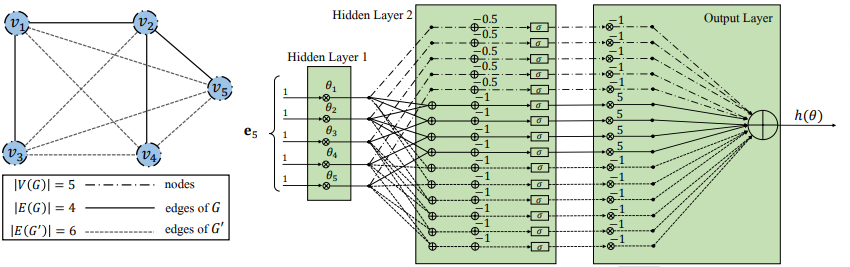
\includegraphics{figures/nn_clique_block_structure.png}
    \caption{An example of graph $G = (V = {v_1, v_2, v_3, v_4, v_5}, E =
{(v_1, v_2), (v_1, v_3), (v_2, v_4), (v_2, v_5)})$ and its dNN construction h for the MIS problem
by leveraging the duality between MIS and MC.
}
    \label{fig:dnn_clique_scheme}
\end{figure}

\section{Analysis of the large graphs}

Many techniques have been developed before to handle large-scale graphs for the MIS problem, such as the linear programming (LP) reduction, elimination of pendant vertices, and other heuristics as reported in \cite{butenko_applications} and used in some of the most recent state-of-the-art approaches. However, as mentioned in \cite{redumis}, these methods are only relevant to sparse graphs.

This inspires us to focus on creating a reduction method that is not dependent on the density or other properties of the graph. When handling big graphs, the suggested method detailed below makes use of dNNs, built on reduced subgraphs. This is especially helpful when optimizing the parameters of one dNN representing the complete graph necessitates a significant amount of storage and processing. 

To divide the graph into communities, which are made up of vertices with dense connections inside same community and sparser connections between communities, we perform Louvain community detection algorithm \cite{Yang2016}. 

The advancement of modularity in the algorithm serves as the model for this community discovery technique. The relative density of edges within communities compared to edges outside communities is measured using a scale called modularity, which ranges from 0.5 (non-modular clustering) to 1 (completely modular clustering). The best potential clustering of the nodes in a given network is achieved by optimizing this value, according to theory. Heuristic methods are utilized instead since it is difficult to iterate the nodes into groups across all potential configurations. In the Louvain Method of community discovery, each tiny community is initially grouped into one node and the first step is repeated until small communities are discovered by improving modularity locally on all nodes. The approach is comparable to an earlier approach developed by Clauset, Newman, and Moore that links communities whose merger results in the greatest gain in modularity.

Then, for the subgraph induced by each community separately, we generate a MIS using Algorithm \ref{alg:neural_network}. 

Let $C_i, i\in[r]$ be the set of nodes in community $i$, where $r$ - total quantity of communities in \graphG found by the community detection algorithm. For each $C_i$ we induce \graphG by $C_i$, $G_i=G[C_i]$. The union of these sets is the set $B = \bigcup_{i \in [r]} \mathcal{I_i}$
When all the communities are processed we obtain set of MIS $U = I$. Because there may be edges connecting nodes in the solution sets of two different communities, it should be noted that $B$ is typically not an independent set with respect to \graphG.

Thus, we call these edges forbidden and should replace or remove them from the solution.
Let's denote the inter-cluster edges:
\begin{equation}
    R = \{(u,v)\in E | u \in C_i, v \in C_j, i\neq j\}
\end{equation}

then, we can describe forbidden edges:
\begin{equation}
    F = \{(u,v) \in R | u \in \mathcal{I}_i, v \in \mathcal{I}_j, i \neq j\}
\end{equation}

We must handle every node having an edge in the set $F$ in order to get a MIS w.r.t. \graphG. In order to achieve this, we use the procedure below, which processes each pair in $F$ until an IS is obtained w.r.t. \graphG. Firstly, we choose a pair $(u, v) \in F$, and then determine if each node $q \in \{u, v\}$ may be substituted by a node in its neighborhood. A vertex $w \in N(q)$, is potential replacement if it is 1-tight, meaning that $|B\cap N(w)| = 1$. If neither $u$ nor $v$ can be replaced, the node in $F$ with the most repeats is eliminated. This procedure is continuing until the set $F$ is empty. Algorithm \ref{alg:forbiden_nodes_removal} provides the complete process. 

\begin{algorithm}
\caption{Forbidden nodes removal}\label{alg:forbiden_nodes_removal}
\begin{algorithmic}
\State \textbf{Input:}\graphG, $B$, $F$
\State \textbf{Output:} IS $\mathcal{I} on G$
\State \textbf{initialize} $\mathcal{I} = B$
\While{$F \neq \varnothing$}
    \State \textbf{select} a pair $(u,v) \in F,$ \textbf{initilize} ReplacementFlag = 0
    \State \textbf{for all} $q \in \{u,v\}$
    \If {$\exists w \in N(q)$ \textbf{s.t.} $|\mathcal{I}\cap N(w)| = 1$}
        \State \textbf{replace} $q$ by $w$, that is $\mathcal{I} \leftarrow \mathcal{I} \ \{q\}, \mathcal{I}\leftarrow \mathcal{I} \cup \{w\}$
        \State \textbf{update} $F$, ReplacementFlag = 1
        \State \textbf{break for}
    \EndIf
    \If {ReplacementFlag = 0 (no replacement is found)}
        \State \textbf{remove} either $u$ or $v$ depending on their repetitions in $F$
        \State \textbf{update} $\mathcal{I}$ and $F$
    \EndIf
\EndWhile
\end{algorithmic}
\end{algorithm}

Assuming that the resulting set $I$ is just an IS with respect to \graphG, we can create a MIS by applying Algorithm \ref{alg:neural_network} to the subgraph that is induced by nodes that are not part of the solution nor its neighborhood.
More strictly, result is updated as 
\begin{equation}
    \mathcal{I} \leftarrow \mathcal{I} \cup \text{dNN}(G[V\textbackslash(\mathcal{I} \cup N(\mathcal{I}))], \alpha)
\end{equation}

Example of the resulting independent sets for different small graphs can be found on figure \ref{figure:graphs_examples}
\begin{figure}
    \centering
  \begin{subfigure}{\linewidth}
  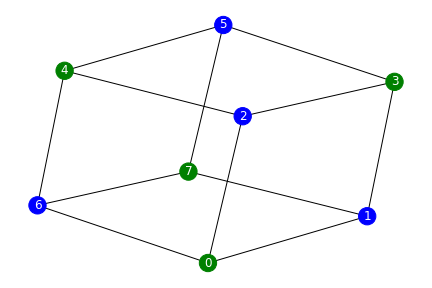
\includegraphics[width=.4\linewidth]{figures/small_graphs/1.png}
  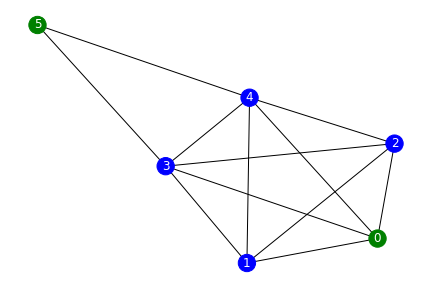
\includegraphics[width=.4\linewidth]{figures/small_graphs/2.png}
  \end{subfigure}\par\medskip
  \begin{subfigure}{\linewidth}
  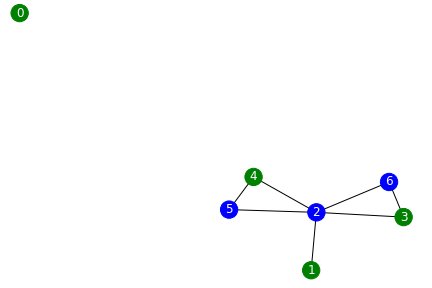
\includegraphics[width=.4\linewidth]{figures/small_graphs/3.png}
  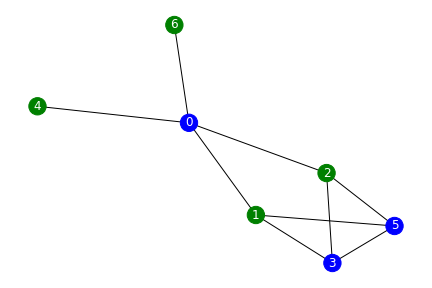
\includegraphics[width=.4\linewidth]{figures/small_graphs/4.png}
  \end{subfigure}\par\medskip
  \begin{subfigure}{\linewidth}
  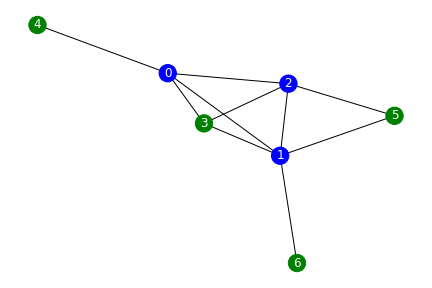
\includegraphics[width=.4\linewidth]{figures/small_graphs/5.png}
  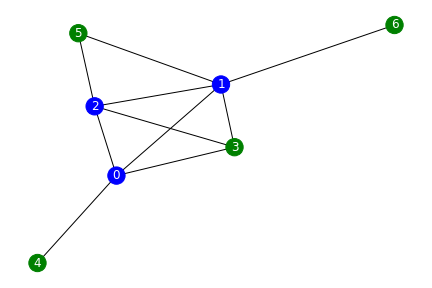
\includegraphics[width=.4\linewidth]{figures/small_graphs/6.png}
  \end{subfigure}\par\medskip
  \caption{Examples of MIS found for small graphs by the dNN algorithm. Vertices that are included to MIS are colored with green} \label{figure:graphs_examples}
\end{figure}

